%%%%%%%%%%%%%%%%%%%%%%%%%%%%%%%%%%%%%%%%%
% Cleese Assignment (For Students)
% LaTeX Template
% Version 2.0 (27/5/2018)
%
% This template originates from:
% http://www.LaTeXTemplates.com
%
% Author:
% Vel (vel@LaTeXTemplates.com)
%
% License:
% CC BY-NC-SA 3.0 (http://creativecommons.org/licenses/by-nc-sa/3.0/)
% 
%%%%%%%%%%%%%%%%%%%%%%%%%%%%%%%%%%%%%%%%%

%----------------------------------------------------------------------------------------
%	PACKAGES AND OTHER DOCUMENT CONFIGURATIONS
%----------------------------------------------------------------------------------------

\documentclass[11pt]{article}
\usepackage{float}

\usepackage[printwatermark]{xwatermark}
\newwatermark[allpages,color=gray!50,angle=45,scale=2.5,xpos=-5,ypos=-5]{Mohammad Hadi}

%%%%%%%%%%%%%%%%%%%%%%%%%%%%%%%%%%%%%%%%%
% Cleese Assignment
% Structure Specification File
% Version 1.0 (27/5/2018)
%
% This template originates from:
% http://www.LaTeXTemplates.com
%
% Author:
% Vel (vel@LaTeXTemplates.com)
%
% License:
% CC BY-NC-SA 3.0 (http://creativecommons.org/licenses/by-nc-sa/3.0/)
% 
%%%%%%%%%%%%%%%%%%%%%%%%%%%%%%%%%%%%%%%%%

%----------------------------------------------------------------------------------------
%	PACKAGES AND OTHER DOCUMENT CONFIGURATIONS
%----------------------------------------------------------------------------------------

\usepackage{lastpage} % Required to determine the last page number for the footer

\usepackage{graphicx} % Required to insert images

\setlength\parindent{0pt} % Removes all indentation from paragraphs

\usepackage[most]{tcolorbox} % Required for boxes that split across pages

\usepackage{booktabs} % Required for better horizontal rules in tables

\usepackage{listings} % Required for insertion of code

\usepackage{etoolbox} % Required for if statements

%----------------------------------------------------------------------------------------
%	MARGINS
%----------------------------------------------------------------------------------------

\usepackage{geometry} % Required for adjusting page dimensions and margins

\geometry{
	paper=a4paper, % Change to letterpaper for US letter
	top=3cm, % Top margin
	bottom=3cm, % Bottom margin
	left=2.5cm, % Left margin
	right=2.5cm, % Right margin
	headheight=14pt, % Header height
	footskip=1.4cm, % Space from the bottom margin to the baseline of the footer
	headsep=1.2cm, % Space from the top margin to the baseline of the header
	%showframe, % Uncomment to show how the type block is set on the page
}

%----------------------------------------------------------------------------------------
%	FONT
%----------------------------------------------------------------------------------------

\usepackage[utf8]{inputenc} % Required for inputting international characters
\usepackage[T1]{fontenc} % Output font encoding for international characters

\usepackage[sfdefault,light]{roboto} % Use the Roboto font

%----------------------------------------------------------------------------------------
%	HEADERS AND FOOTERS
%----------------------------------------------------------------------------------------

\usepackage{fancyhdr} % Required for customising headers and footers

\pagestyle{fancy} % Enable custom headers and footers

\lhead{\small\assignmentClass\ifdef{\assignmentClassInstructor}{\ (\assignmentClassInstructor):}{}\ \assignmentTitle} % Left header; output the instructor in brackets if one was set
\chead{} % Centre header
\rhead{\small\ifdef{\assignmentAuthorName}{\assignmentAuthorName}{\ifdef{\assignmentDueDate}{Due\ \assignmentDueDate}{}}} % Right header; output the author name if one was set, otherwise the due date if that was set

\lfoot{} % Left footer
\cfoot{\small Page\ \thepage\ of\ \pageref{LastPage}} % Centre footer
\rfoot{} % Right footer

\renewcommand\headrulewidth{0.5pt} % Thickness of the header rule

%----------------------------------------------------------------------------------------
%	MODIFY SECTION STYLES
%----------------------------------------------------------------------------------------

\usepackage{titlesec} % Required for modifying sections

%------------------------------------------------
% Section

\titleformat
{\section} % Section type being modified
[block] % Shape type, can be: hang, block, display, runin, leftmargin, rightmargin, drop, wrap, frame
{\Large\bfseries} % Format of the whole section
{\assignmentQuestionName~\thesection} % Format of the section label
{6pt} % Space between the title and label
{} % Code before the label

\titlespacing{\section}{0pt}{0.5\baselineskip}{0.5\baselineskip} % Spacing around section titles, the order is: left, before and after

%------------------------------------------------
% Subsection

\titleformat
{\subsection} % Section type being modified
[block] % Shape type, can be: hang, block, display, runin, leftmargin, rightmargin, drop, wrap, frame
{\itshape} % Format of the whole section
{(\alph{subsection})} % Format of the section label
{4pt} % Space between the title and label
{} % Code before the label

\titlespacing{\subsection}{0pt}{0.5\baselineskip}{0.5\baselineskip} % Spacing around section titles, the order is: left, before and after

\renewcommand\thesubsection{(\alph{subsection})}

%----------------------------------------------------------------------------------------
%	CUSTOM QUESTION COMMANDS/ENVIRONMENTS
%----------------------------------------------------------------------------------------

% Environment to be used for each question in the assignment
\newenvironment{question}{
	\vspace{0.5\baselineskip} % Whitespace before the question
	\section{} % Blank section title (e.g. just Question 2)
	\lfoot{\small\itshape\assignmentQuestionName~\thesection~continued on next page\ldots} % Set the left footer to state the question continues on the next page, this is reset to nothing if it doesn't (below)
}{
	\lfoot{} % Reset the left footer to nothing if the current question does not continue on the next page
}

%------------------------------------------------

% Environment for subquestions, takes 1 argument - the name of the section
\newenvironment{subquestion}[1]{
	\subsection{#1}
}{
}

%------------------------------------------------

% Command to print a question sentence
\newcommand{\questiontext}[1]{
	\textbf{#1}
	\vspace{0.5\baselineskip} % Whitespace afterwards
}

%------------------------------------------------

% Command to print a box that breaks across pages with the question answer
\newcommand{\answer}[1]{
	\begin{tcolorbox}[breakable, enhanced]
		#1
	\end{tcolorbox}
}

%------------------------------------------------

% Command to print a box that breaks across pages with the space for a student to answer
\newcommand{\answerbox}[1]{
	\begin{tcolorbox}[breakable, enhanced]
		\vphantom{L}\vspace{\numexpr #1-1\relax\baselineskip} % \vphantom{L} to provide a typesetting strut with a height for the line, \numexpr to subtract user input by 1 to make it 0-based as this command is
	\end{tcolorbox}
}

%------------------------------------------------

% Command to print an assignment section title to split an assignment into major parts
\newcommand{\assignmentSection}[1]{
	{
		\centering % Centre the section title
		\vspace{2\baselineskip} % Whitespace before the entire section title
		
		\rule{0.8\textwidth}{0.5pt} % Horizontal rule
		
		\vspace{0.75\baselineskip} % Whitespace before the section title
		{\LARGE \MakeUppercase{#1}} % Section title, forced to be uppercase
		
		\rule{0.8\textwidth}{0.5pt} % Horizontal rule
		
		\vspace{\baselineskip} % Whitespace after the entire section title
	}
}

%----------------------------------------------------------------------------------------
%	TITLE PAGE
%----------------------------------------------------------------------------------------

\author{\textbf{\assignmentAuthorName}} % Set the default title page author field
\date{} % Don't use the default title page date field

\title{
	\thispagestyle{empty} % Suppress headers and footers
	\vspace{0.2\textheight} % Whitespace before the title
	\textbf{\assignmentClass:\ \assignmentTitle}\\[-4pt]
	\ifdef{\assignmentDueDate}{{\small Due\ on\ \assignmentDueDate}\\}{} % If a due date is supplied, output it
	\ifdef{\assignmentClassInstructor}{{\large \textit{\assignmentClassInstructor}}}{} % If an instructor is supplied, output it
	\vspace{0.32\textheight} % Whitespace before the author name
}
 % Include the file specifying the document structure and custom commands

%----------------------------------------------------------------------------------------
%	ASSIGNMENT INFORMATION
%----------------------------------------------------------------------------------------

% Required
\newcommand{\assignmentQuestionName}{Experiment} % The word to be used as a prefix to question numbers; example alternatives: Problem, Exercise
\newcommand{\assignmentClass}{Electrical Circuits Lab (Taught by Mohammad Hadi)\\Manual 7 (Due on DDD.,\ mmm.\ dd,\ yyyy)} % Course (Lecturer)\\Assignment (Due date)
\newcommand{\assignmentTitle}{} % Assignment title or name
\newcommand{\assignmentAuthorName}{Student Names\\Student Numbers} % Student name\\Student number
%----------------------------------------------------------------------------------------

\begin{document}
\textbf{Frequency response is a measurable concept that can be used to experimentally and analytically describe a circuit. In this experiment, you become familiar with the frequency response of first- and second-order circuits.
}
%----------------------------------------------------------------------------------------
%	TITLE PAGE
%----------------------------------------------------------------------------------------

\assignmentSection{Mandatory Experiments}

%----------------------------------------------------------------------------------------
%	QUESTION 1
%----------------------------------------------------------------------------------------

\begin{question}

\questiontext{Build the circuit shown in Fig. \ref{fig:cir1} on a breadboard. Instead of using a physical switch, connect or disconnect the supply wire.}

\begin{figure}[H]
\centering
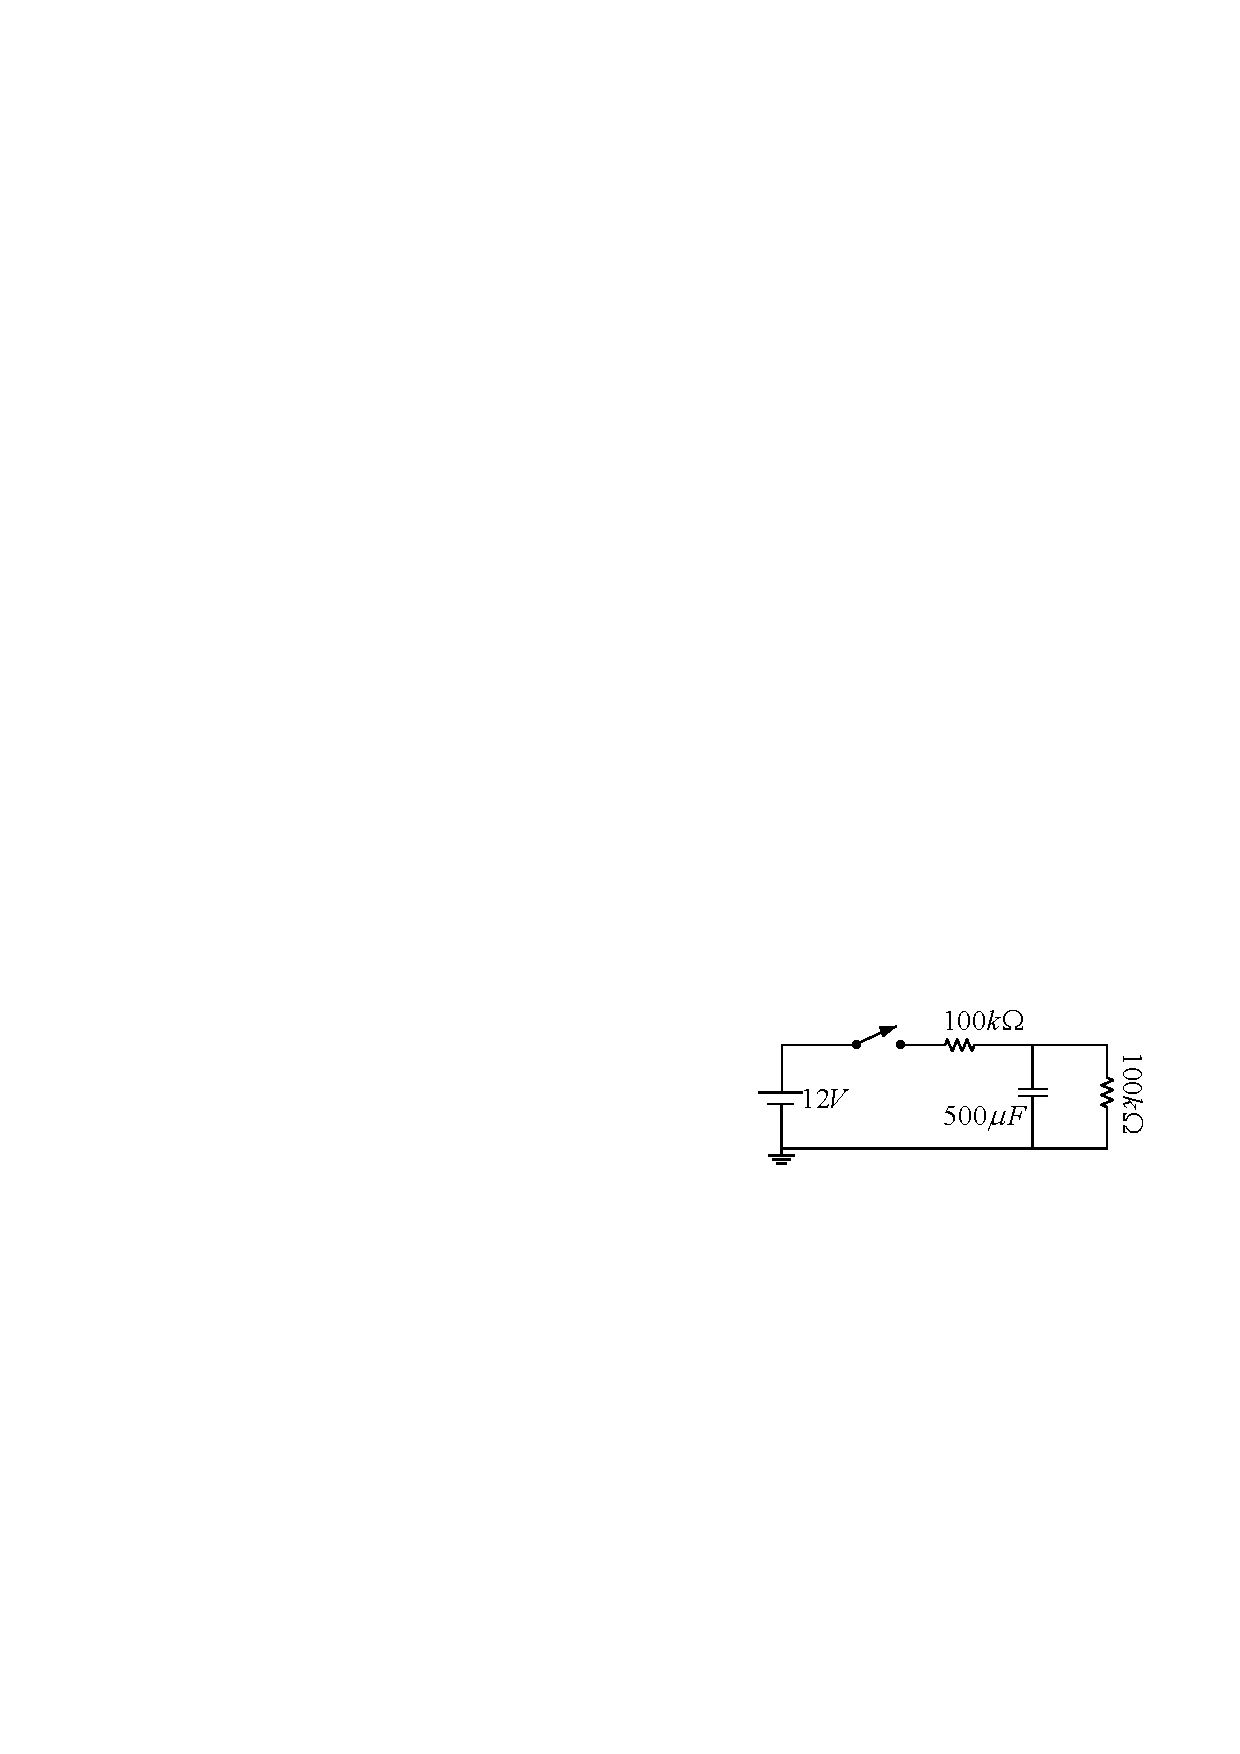
\includegraphics[scale=1.2,angle=0]{Fig/cir1.pdf}
\caption{An RC circuit.} \label{fig:cir1}
\end{figure}

%--------------------------------------------
\begin{subquestion}{Connect and disconnect the supplu wire to see the capacitor voltage response on the oscilloscope screen. Discuss the results.} 
\answer{}
\end{subquestion}

%--------------------------------------------
\begin{subquestion}{Measure the time constant of the circuit and compare it to its analytical counterpart.} 
\answer{}
\end{subquestion}

%--------------------------------------------
\begin{subquestion}{Decrease the supply voltage to $5$ V and redo the previous parts.} 
\answer{}
\end{subquestion}


\end{question}

%----------------------------------------------------------------------------------------
%	QUESTION 2
%----------------------------------------------------------------------------------------

\begin{question}

\questiontext{Build the circuit shown in Fig. \ref{fig:cir2} on a breadboard.}

\begin{figure}[H]
\centering
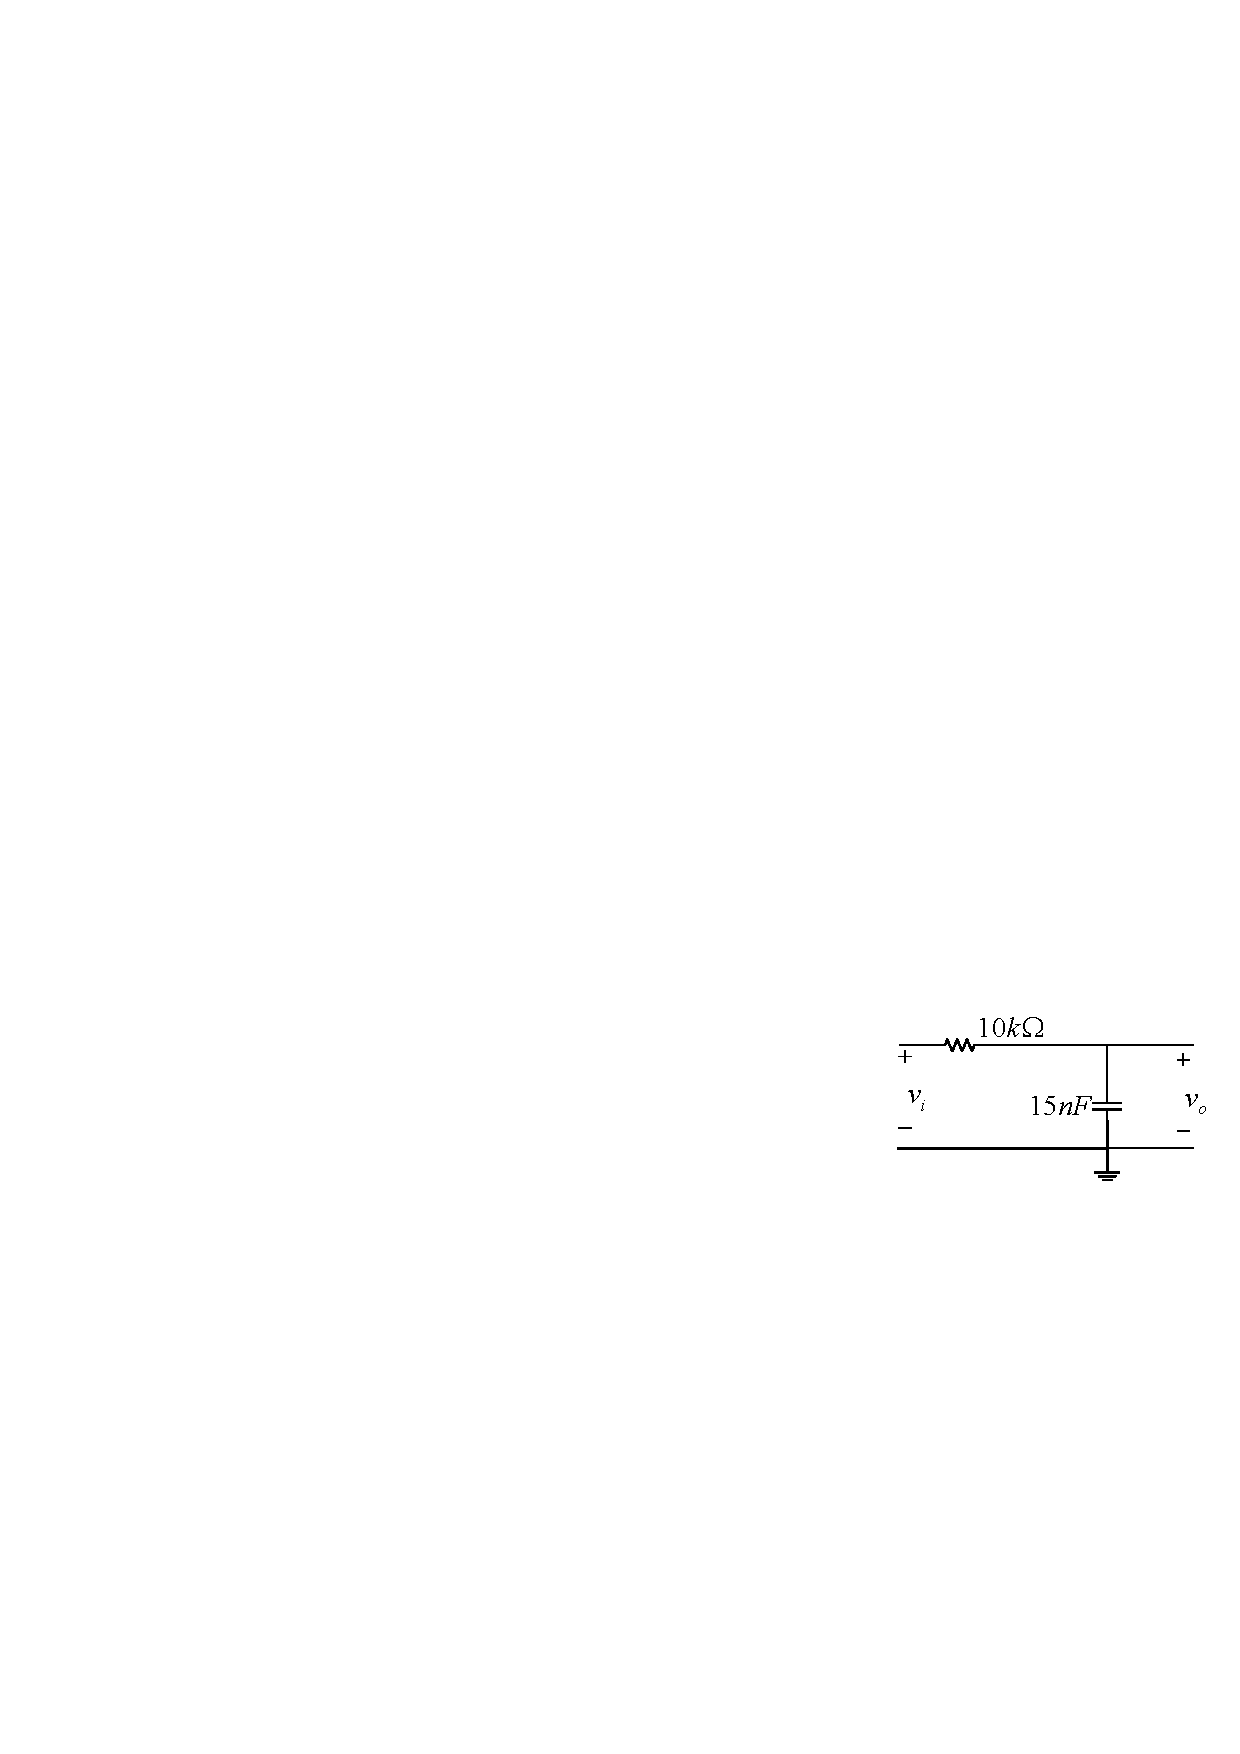
\includegraphics[scale=1.2,angle=0]{Fig/cir2.pdf}
\caption{A lowpass RC circuit.} \label{fig:cir2}
\end{figure}

%--------------------------------------------
\begin{subquestion}{Apply a $1$-V $300$-Hz square wave to the input. See the input and output voltages simultaneously on the oscilloscope screen. Interpret the observations. Obtain the time constant of the circuit.} 
\answer{}
\end{subquestion}

%--------------------------------------------
\begin{subquestion}{Apply a $1$-V sine wave to the input and change its frequency to measure the frequency response of the circuit using interpolation. See the input and output voltages simultaneously on the oscilloscope and discuss the filtering behavior of the circuit.} 
\answer{}
\end{subquestion}


\end{question}

%----------------------------------------------------------------------------------------
%	QUESTION 3
%----------------------------------------------------------------------------------------

\begin{question}

\questiontext{Build the circuit shown in Fig. \ref{fig:cir3} on a breadboard.}

\begin{figure}[H]
\centering
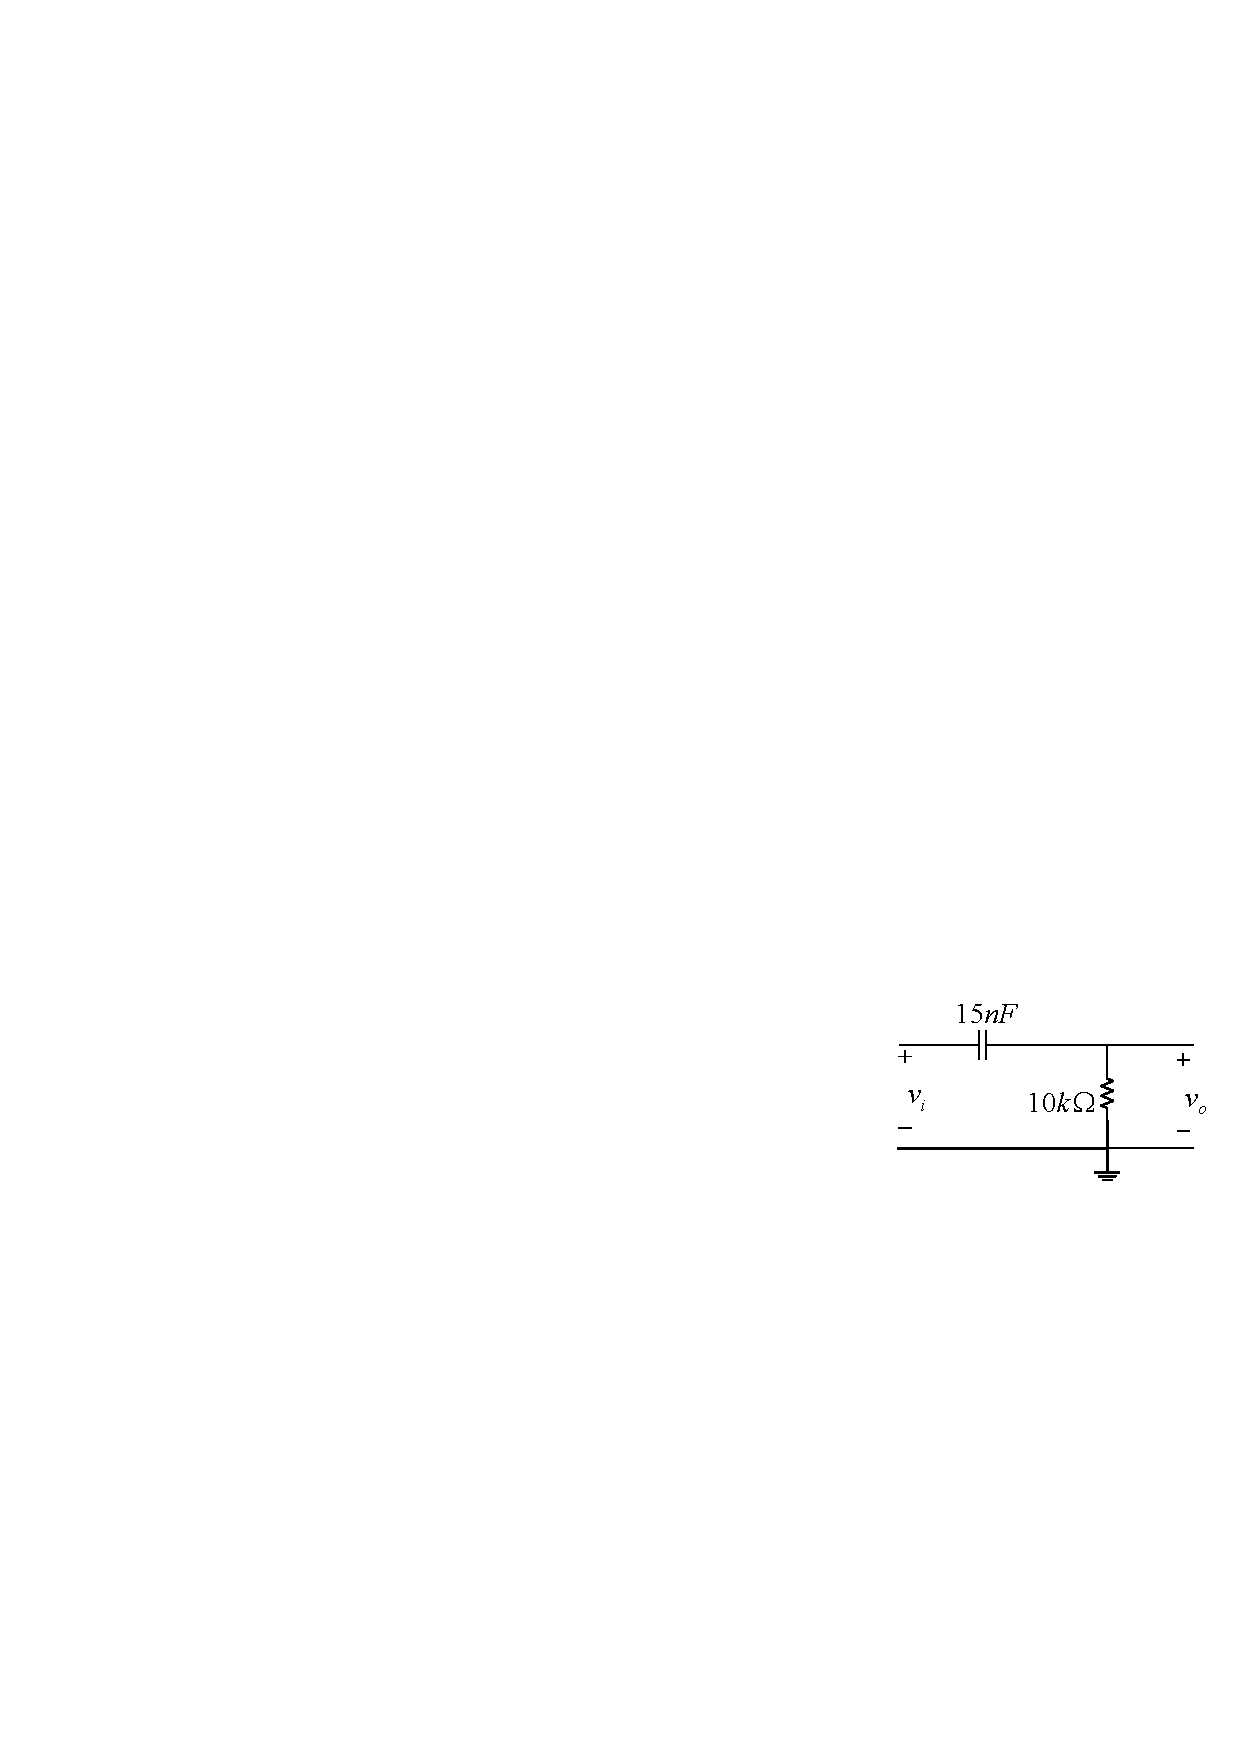
\includegraphics[scale=1.2,angle=0]{Fig/cir3.pdf}
\caption{A highpass RC circuit.} \label{fig:cir3}
\end{figure}

%--------------------------------------------
\begin{subquestion}{Apply a $1$-V $300$-Hz square wave to the input. See the input and output voltages simultaneously on the oscilloscope screen. Interpret the observations. Obtain the time constant of the circuit.} 
\answer{}
\end{subquestion}

%--------------------------------------------
\begin{subquestion}{Apply a $1$-V sine wave to the input and change its frequency to measure the frequency response of the circuit using interpolation. See the input and output voltages simultaneously on the oscilloscope and discuss the filtering behavior of the circuit.} 
\answer{}
\end{subquestion}


\end{question}

%----------------------------------------------------------------------------------------
%	QUESTION 4
%----------------------------------------------------------------------------------------

\begin{question}

\questiontext{Build the circuit shown in Fig. \ref{fig:cir4} on a breadboard.}

\begin{figure}[H]
\centering
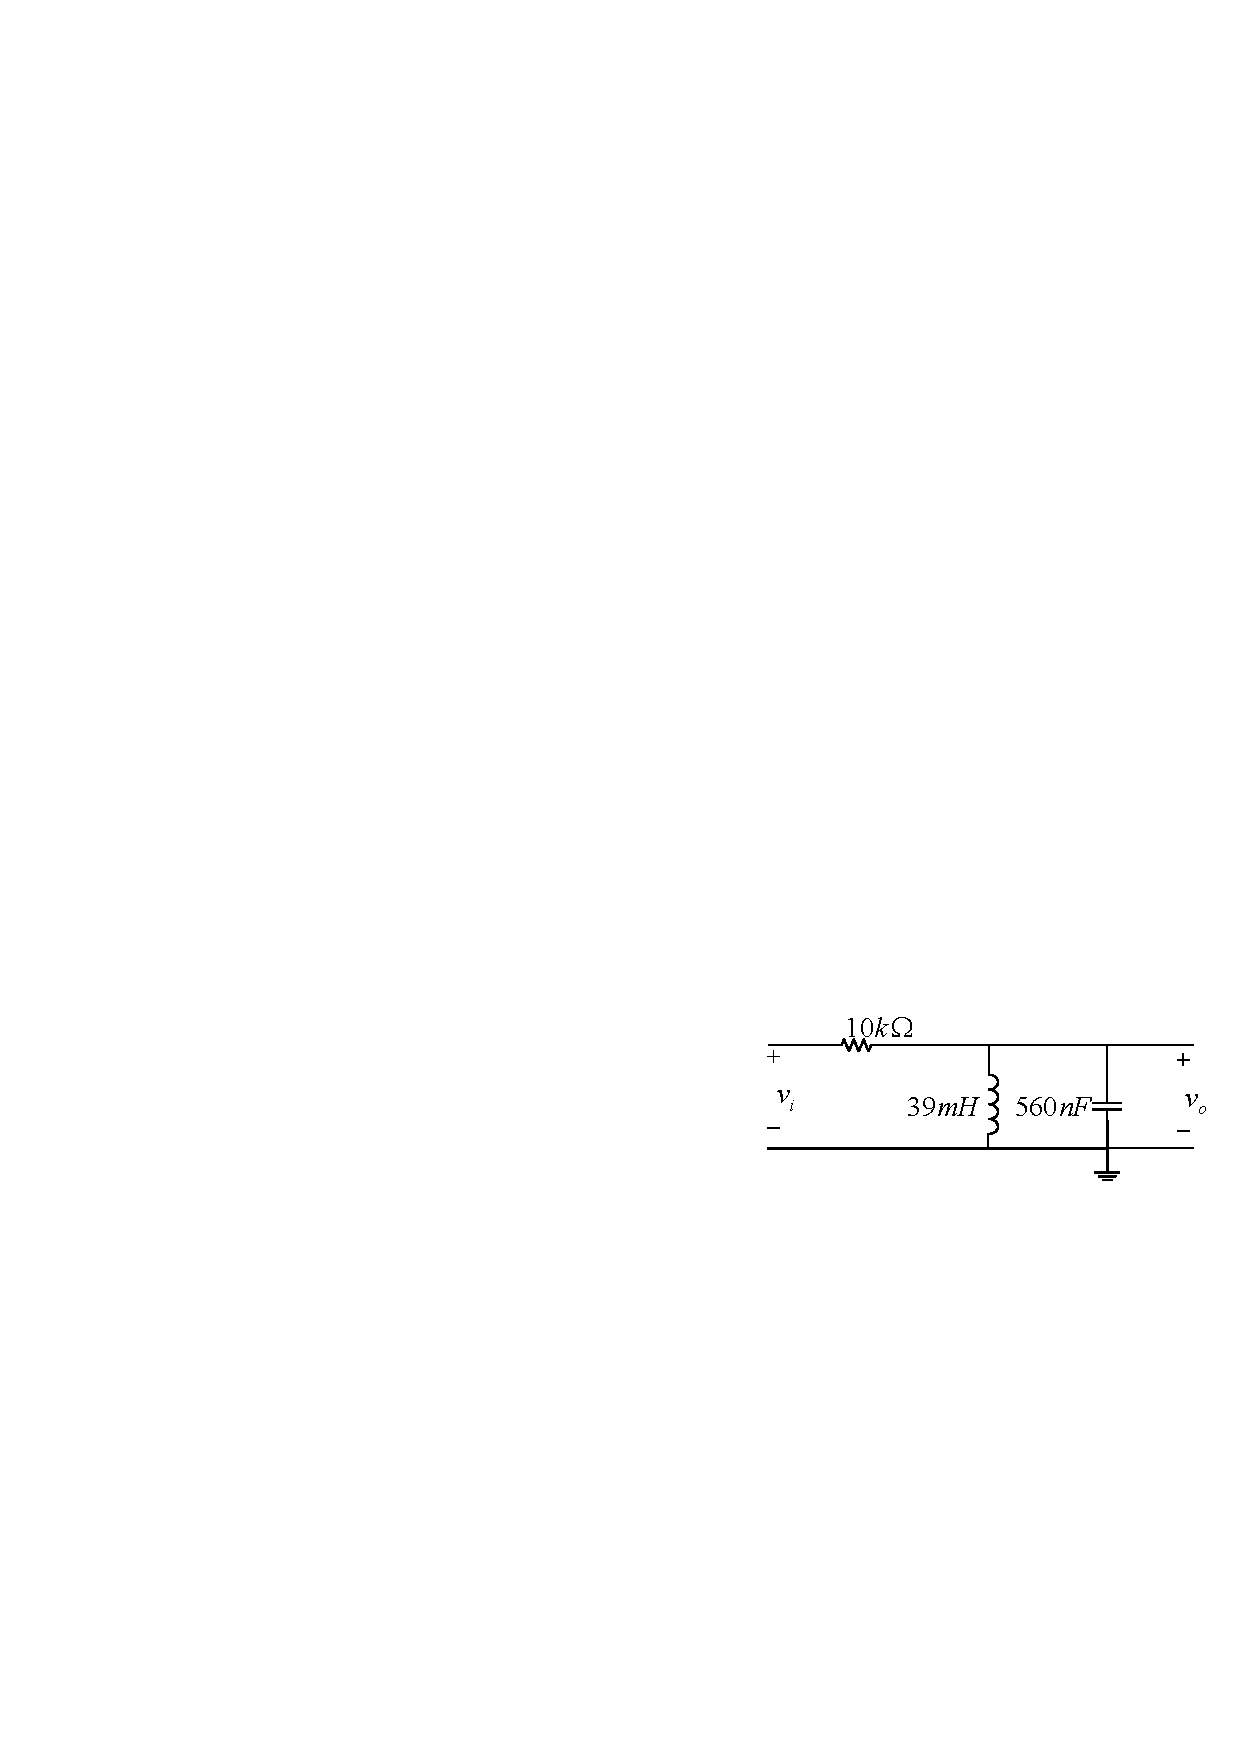
\includegraphics[scale=1.2,angle=0]{Fig/cir4.pdf}
\caption{A bandpass RLC circuit.} \label{fig:cir4}
\end{figure}

%--------------------------------------------
\begin{subquestion}{Apply a $1$-V sine wave to the input and change its frequency from $100$ Hz to $10$ kHz to measure the frequency response of the circuit using interpolation. See the input and output voltages simultaneously on the oscilloscope and discuss the filtering behavior of the circuit.} 
\answer{}
\end{subquestion}

%--------------------------------------------
\begin{subquestion}{Apply a $1$-V square wave to the input and sweep its frequency from $100$ Hz to $10$ kHz. See the input and output voltages simultaneously on an oscilloscope screen. Interpret the observations.} 
\answer{}
\end{subquestion}

\end{question}


\assignmentSection{Bonus Experiments}

%----------------------------------------------------------------------------------------
%	QUESTION 5
%----------------------------------------------------------------------------------------

\begin{question}

\questiontext{The circuit shown in Fig. \ref{fig:Q5} is called Sallen active lowpass filter, where the triangle abstracts an op-amp amplification circuit with the gain $K$.}

\begin{figure}[H] 
\begin{center}
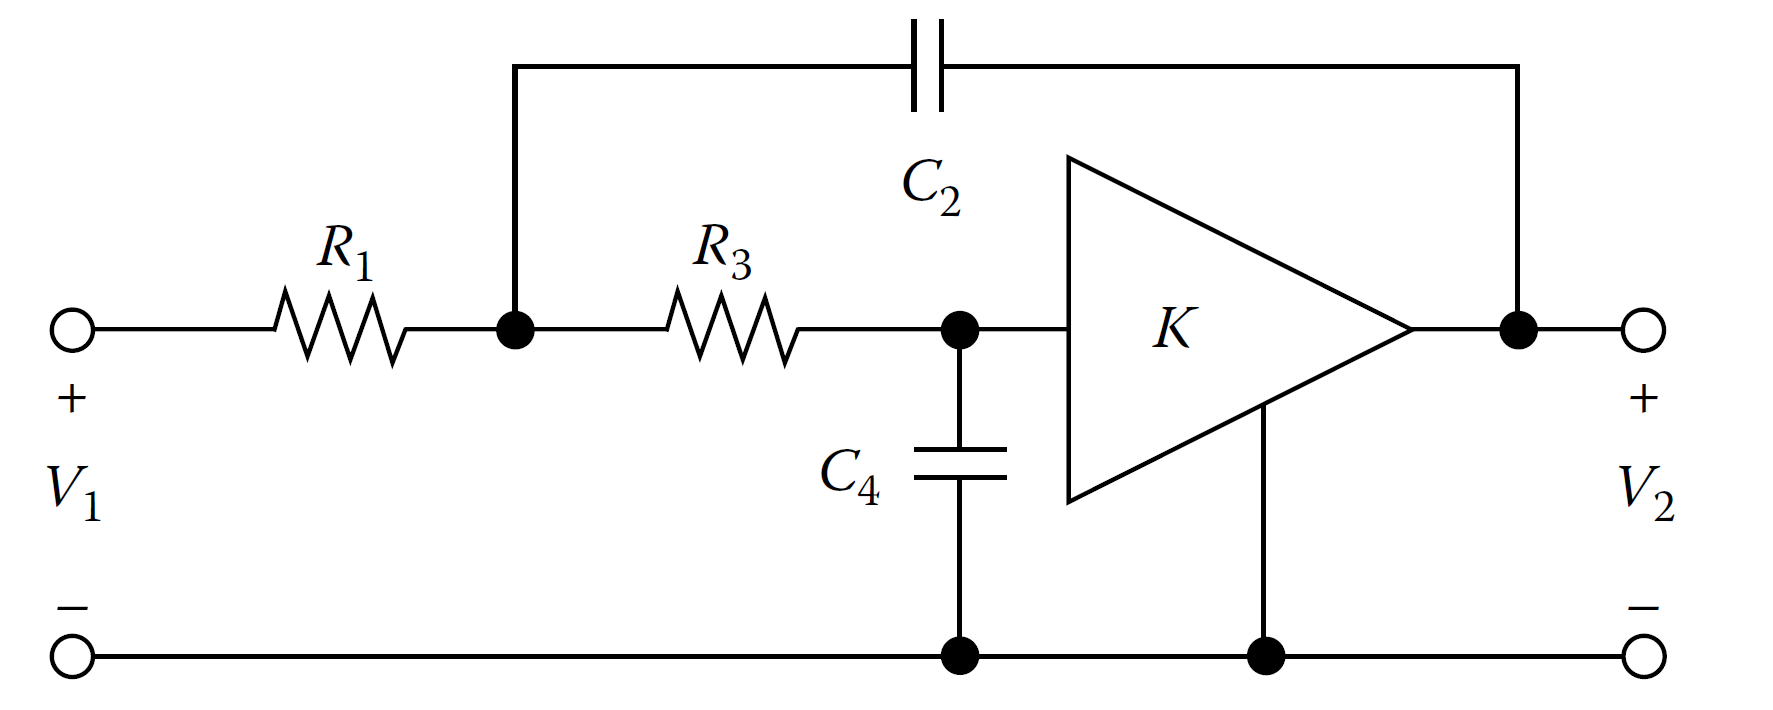
\includegraphics[scale=0.3]{Fig/Q5.png}
\caption{\label{fig:Q5} Sallen active lowpass filter.}
\end{center}
\end{figure}  

%--------------------------------------------
\begin{subquestion}{Calculate the frequency response of the active filter circuit.} 
\answer{}
\end{subquestion}
%--------------------------------------------
\begin{subquestion}{How can the amplifier part be implemented using op-amps?} 
\answer{}
\end{subquestion}
%--------------------------------------------
\begin{subquestion}{What are the advantages of the amplification part? Does it have any impact on the filtering response?} 
\answer{}
\end{subquestion}
%--------------------------------------------
\begin{subquestion}{What are the advantages and disadvantages of such an active filter?} 
\answer{}
\end{subquestion}

\end{question}


%----------------------------------------------------------------------------------------
%	QUESTION 6
%----------------------------------------------------------------------------------------
\begin{question}
\questiontext{The circuit shown in Fig. \ref{fig:Q6} is called biquad active filter. The triangles denote two amplifiers with the gains $-1$ and $2$. The amplifiers may be implemented using inverting and non-inverting op-amp circuits. The admittances $Y_1$, $Y_2$, $Y_3$ and $Y_4$ can be replaced by series or parallel RC circuits. A sample customized configuration is shown in Fig. \ref{fig:Q6_1}. Depending on the configuration, the circuit provides various filtering responses. 
}
\begin{figure}[H] 
\begin{center}
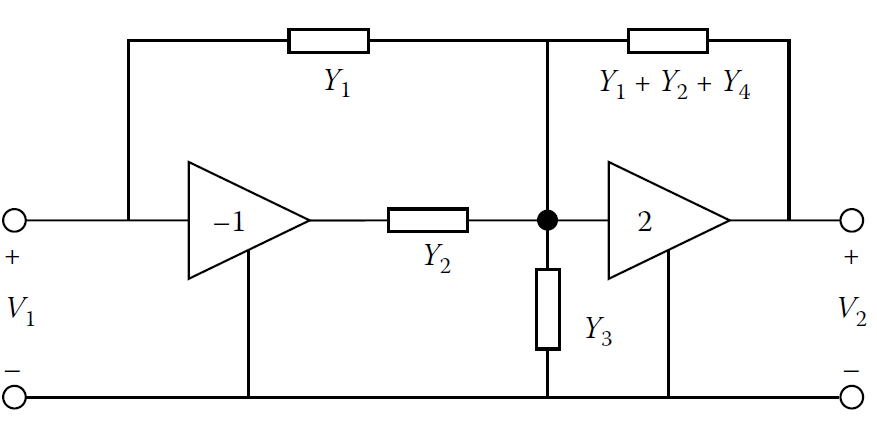
\includegraphics[scale=0.5]{Fig/Q6.png}
\caption{\label{fig:Q6} Biquad active filter.}
\end{center}
\end{figure}  
\begin{figure}[H] 
\begin{center}
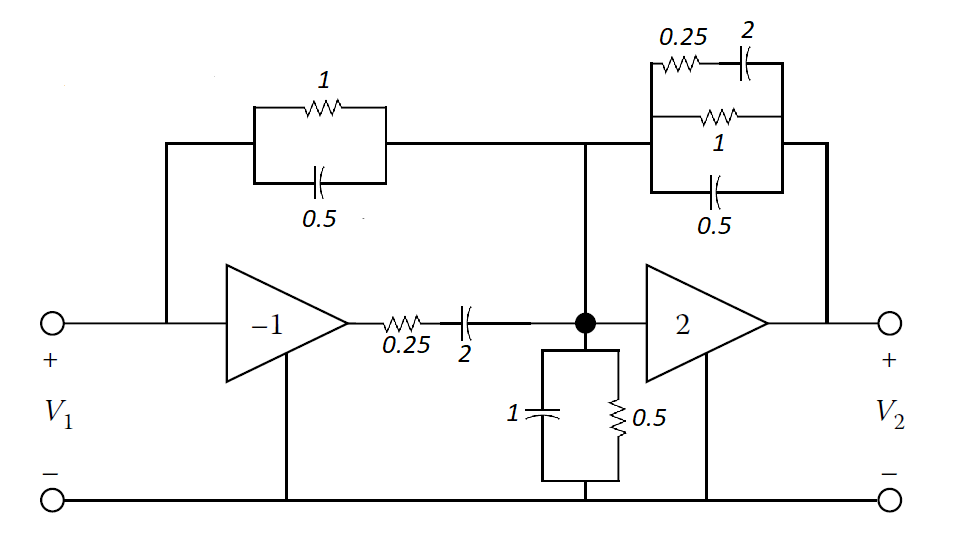
\includegraphics[scale=0.5]{Fig/Q6_1.png}
\caption{\label{fig:Q6_1} A sample customized realization of the biquad active filter.}
\end{center}
\end{figure}


%--------------------------------------------
\begin{subquestion}{Simulate the circuit in PSpice and investigate the filtering response of the circuit for various configurations of $Y_1$, $Y_2$, $Y_3$ and $Y_4$. Especially, demonstrate how the biquad filter can have lowpass, highpass, bandpass, and bandstop frequency responses.}
\answer{}
\end{subquestion}
%--------------------------------------------
\begin{subquestion}{What is an all-pass filter and how can it be implemented using a biquad?} 
\answer{}
\end{subquestion}

\end{question}


%----------------------------------------------------------------------------------------
%	QUESTION 7
%----------------------------------------------------------------------------------------

\begin{question}

\questiontext{Return your work report by filling the \LaTeX template of the manual. Include useful and high-quality images to make the report more readable and understandable.}

\end{question}

%----------------------------------------------------------------------------------------

\end{document}
